\chapter{Proton-proton interactions and their simulation}
\label{chap:event:MC}
\glsunset{atlas}

\Gls{pp} interactions at the \gls{lhc} are complex processes that span very different energy scales. 
In order to interpret the experimental data it is essential to develop a good understanding of the physics involved in the \gls{pp} collisions, and the ability to simulate the various processes is also crucial to be able to compare the observed data with the patterns predicted by the theory.
Section \ref{sec:ppint} focuses on the description of our understanding of a \gls{pp} collision, while Section \ref{sec:eventsimul} 
discusses the event-simulation process; 
the main \gls{mc} generators used in the \gls{atlas} Collaboration are described in Section \ref{sec:mcgen}, and Section \ref{sec:detsim} touches briefly on the topics of detector simulation and data-driven corrections.



\section{p-p interactions}
\label{sec:ppint}

In hard-scattering processes, where the momentum transfer is much higher than the proton mass \cite{Butterworth:2012fj}, 
a \gls{pp} collision is easier to understand in terms of interactions between the constituents of the protons, quarks and gluons, 
collectively referred to as partons. A schematic view of \gls{pp} event is shown in Fig. \ref{fig:sim:pp2}. In this particular example, the interaction between a quark and a gluon leads to a final state with a Z boson and jets. 

\begin{figure}[h]
\begin{center}
%  \subfigure[]{
%    \label{fig:Comb_syst:pt}
    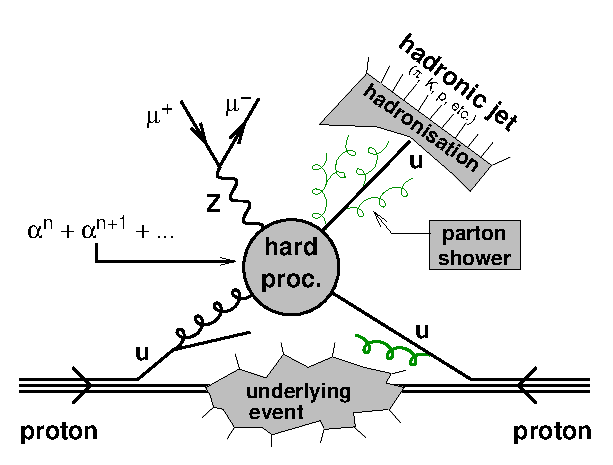
\includegraphics[width=0.58\textwidth]{figures/simul/ppcoll2}
%  }
\end{center}
 \caption{Schematic representation of a \gls{pp}, involving a quark-gluon scattering that leads to a final state consisting of a Z boson and a hard jet. Figure from Ref. \cite{Butterworth:2012fj}.}
  \label{fig:sim:pp2}
\end{figure}

As in can be appreciated from the figure, the hard process, which can be computed in perturbation theory, takes place between two of the proton's partons; the probability that a gluon or a specific quark type takes part in the hard scattering is described by the \glspl{partdf}, discussed in Section \ref{sec:ppint:hardscatter}. If the products of the hard scattering are quarks or gluons, they first of all loose energy by radiating other gluons (which in turn can generate quark-antiquark pairs through gluon splitting) in the process of parton shower;
successively they evolve into stable hadrons in the lower-energy hadronization process, which we can describe only through phenomenological models.
This picture is further complicated by the fact that also initial-state quarks and gluons can radiate. Also, the other partons not contributing to the hard scattering can interact, originating what is referred to as the underlying event. 

\subsection{Factorization theorem}
\label{sec:ppint:hardscatter}

The hard scattering between the partons inside the proton takes place in a kinematic regime where the strong coupling constant, $\alpha_s$, 
is small and therefore the partonic cross-sections can be computed in perturbation theory. 
Thanks to the factorization theorem \cite{doi:10.1146}, the generic production cross-section for a final state $X$ can be expressed in terms of the partonic cross-section $\hat\sigma$ as:

\begin{equation}
  \sigma(pp\rightarrow X) = \sum_{i,j} \int dx_1 dx_2\, 
     f_{i}(x_1,\mu_F^2)\, f_{j}(x_2,\mu_F^2)\, 
     \hat\sigma_{ij\rightarrow X}(x_1 x_2 s, \mu_R^2, \mu_F^2) \; .
  \label{eq:general-cross-section}
\end{equation}
The $i$ and $j$ indexes run over all possible partons, and $f_{i}(x_1,\mu_F^2)$ is the \gls{partdf} for the parton of type $i$, representing 
the distribution of probability for that parton to carry a fraction $x_1$ of the proton momentum when the proton is probed at a scale $\mu_F$
(factorization scale). $\hat\sigma_{ij\rightarrow X}$ is the partonic cross-section, computed at the partonic center of mass energy \cmpart;   
it has to be noted that \cmpart is lower than the total center of mass energy, as 
$\cmpart = x_1 \times x_2 \times s$, 
where $x_1$ and $x_2$ are the fraction of the proton momentum that is carried by each of the two partons.
Although the partonic cross-section depends on $\mu_F$ and on the renormalization scale $\mu_R$, 
which is the scale used for the evaluation of $\alpha_s$, 
when considered at all orders in perturbative \gls{qcd} this dependence disappears.
Higher-order calculations exhibit a reduced scale dependence, and are therefore used whenever available. 


% factorization theorem 


%\begin{figure}[h]
%\begin{center}
%  \subfigure[]{
%    \label{fig:Comb_syst:pt}
%    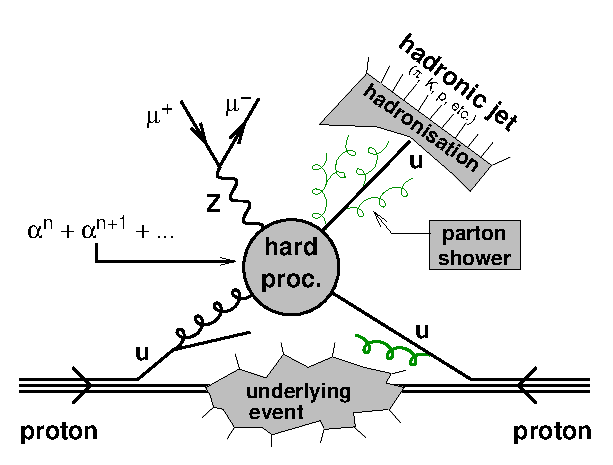
\includegraphics[width=0.48\textwidth]{figures/simul/ppcoll2}
%  }
%    \subfigure[]{
%    \label{fig:Comb_syst:pt}
%    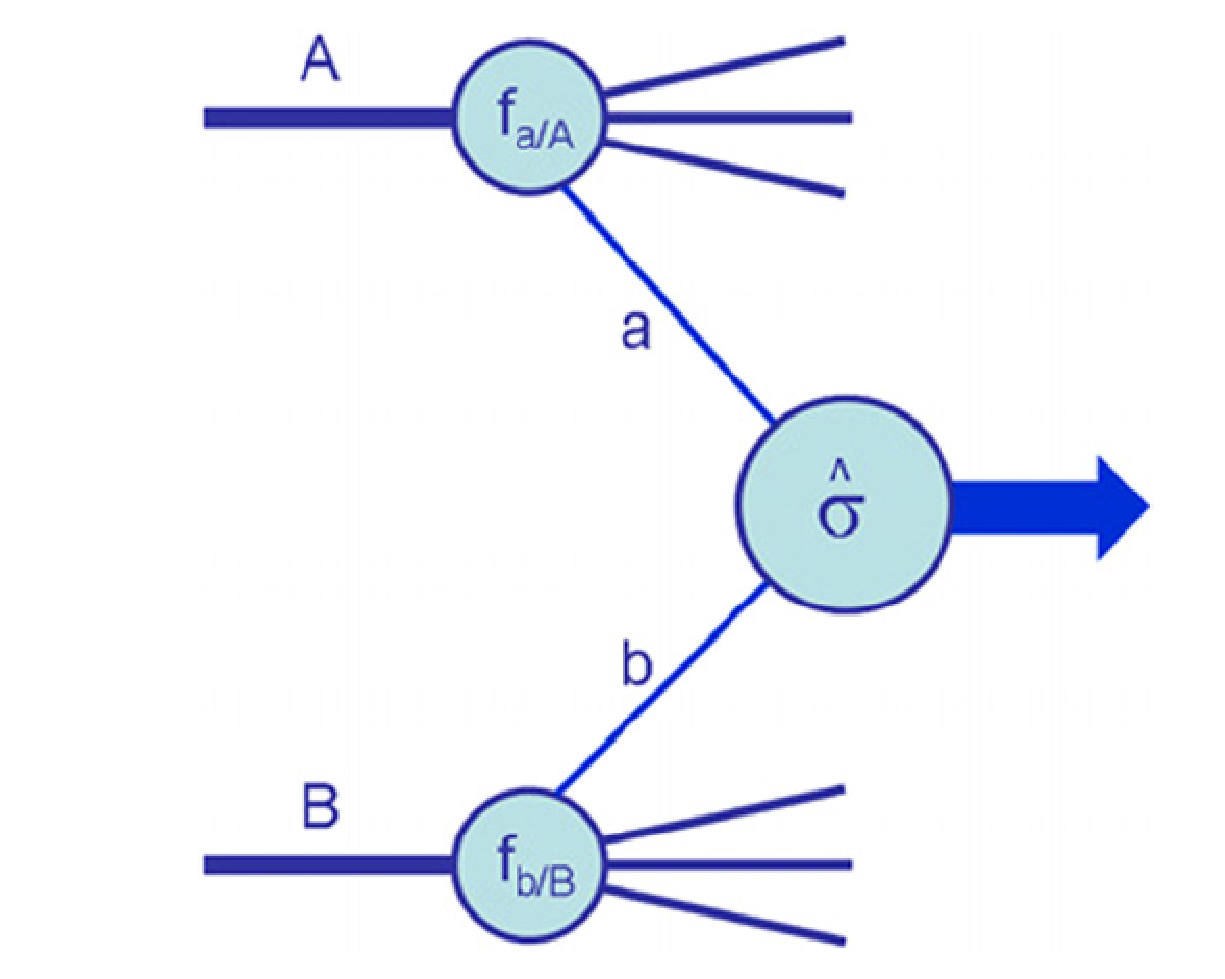
\includegraphics[width=0.48\textwidth]{figures/simul/ppcoll}
%  }
%\end{center}
% \caption{Diagrammatic structure of a generic hard-scattering process. Figure from Ref. \cite{Campbell:2006wx}.}
%  \label{fig:sim:pp}
%\end{figure}

\subsection{Parton density functions}
\label{sec:protpdf}

The partons inside the proton can not be observed as free particles, and therefore their \glspl{partdf} can not be computed with
perturbative \gls{qcd}. In particular, for a given scale, it is not possible to predict theoretically the probability distribution 
of the parton's momentum fraction. Instead, once the \glspl{partdf} are known at a certain scale, their energy evolution is 
determined by the equations derived independently by Dokshitzer \cite{Dokshitzer:1977sg} , Gribov and Lipatov \cite{Gribov:1972ri}, and Altarelli and Parisi \cite{ALTARELLI1977298} (DGLAP equations):

\begin{equation}
\begin{aligned}
\frac{\partial q(x,Q^2)}{\partial {\rm log}Q^2}~&=~\frac{\alpha_s}{2\pi}~\left( P_{qq} \otimes q~+~P_{qg} \otimes g \right) \, ,\\
\frac{\partial g(x,Q^2)}{\partial {\rm log}Q^2}~&=~\frac{\alpha_s}{2\pi}~\left( \sum_i P_{gq} \otimes (q_i+\bar{q}_i)~+~P_{gg} \otimes g \right) \; .
\label{eq:glap1}
\end{aligned}
\end{equation}

\noindent In the expressions above, $q(x,Q^2)$ and $g(x,Q^2)$ denote the quark and gluon \glspl{partdf} respectively, 
$P_{ij}$ describes the $i \to j$ parton splitting function
and $\otimes$ is a symbol for the convolution integral:
\begin{equation}
P \otimes f \equiv \int^1_x\frac{dy}{y}f_q(y)~P\left(\frac{x}{y}\right).
\end{equation}

As mentioned above, the \glspl{partdf} have to be determined experimentally. This is done by several collaborations through fits (with typically 10 to 30 parameters) to data from \gls{dis} experiments. As an example, Figure \ref{fig:sim:pp} shows the \gls{nlo} \glspl{partdf} obtained by the MSTW Collaboration for two different scales, Q$^2$ = 10 GeV$^2$ and Q$^2$ = 10$^4$ GeV$^2$. As can be appreciated, with the increase of Q$^2$, the shape of the \glspl{partdf} changes to favor lower $x$ values. At low $x$ values the gluon \gls{partdf} is dominating (and this effect increases with Q$^2$), while for high $x$ values the \glspl{partdf} of the valence quarks are more relevant.

\begin{figure}[h]
\begin{center}
    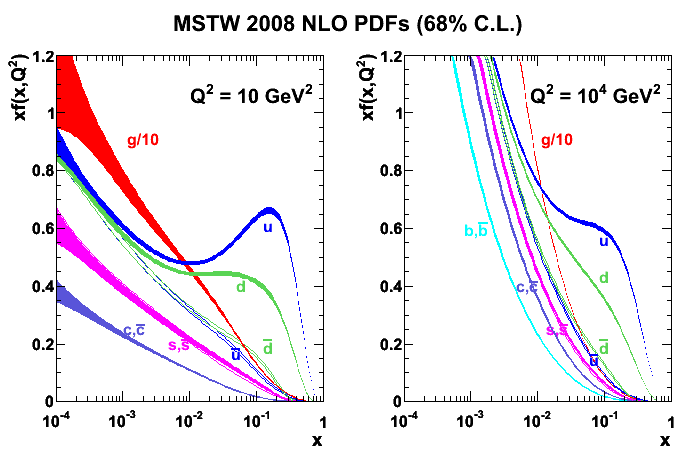
\includegraphics[width=0.8\textwidth]{figures/simul/pdf}
\end{center}
\caption{MSTW 2008 \gls{nlo} \glspl{partdf} at Q$^2$ = 10 GeV$^2$ and Q$^2$ = 10$^4$ GeV$^2$. Figure from Ref. \cite{Martin:2009iq}.}
 \label{fig:sim:pp}
\end{figure}


\section{Event simulation}
\label{sec:eventsimul}

The main steps in the simulation of a \gls{pp} collision consists of:
\begin{itemize}
\item Computation of the \glspl{me} for the hard process.
\item \Gls{psh} evolution and matching between \gls{psh} and \glspl{me}.
\item Hadronization and decay of unstable particles.
\item Simulation of the underlying event and pileup.
\end{itemize}
In the next sections, each step is summarized in its main features.

\subsection{Matrix element}

As discussed e.g. in Ref \cite{Skands:2011pf}, the partonic cross-section for the production of the final state $X$ starting from the partons $i$ and $j$, necessary to compute
Equation \ref{eq:general-cross-section}, can be expressed at all orders as:
\begin{equation}
\hat\sigma_{ij\rightarrow X} = \sum_{k=0}^\infty \int d\Phi_{X+k} | \sum_{l=0}^\infty \mathcal{M}_{X+k}^{(l)}|^2 \; .
\label{eq:xsec_matrix}
\end{equation}
\noindent In this expression, the index $k$ denotes the number of final-state quarks and gluons produced in addition to $X$ (legs) and $\mathcal{M}_{X+k}^{(l)}$
the amplitude to produce the final state $X+k$ computed with $l$ virtual loops. To compute a cross-section is not possible to extend these sums to infinity, and the number of extra partons and the number of loops identify the 
perturbative order of the cross-section. In particular:
\begin{itemize}
\item The lowest possible order for the calculation of $\hat{\sigma}_{ij \rightarrow X}$ is the \gls{lo}, where $k=l=0$.
\item $l=0$, $k=n$ represents the \gls{lo} computation for the production of $X$ + $n$ jets.
\item $k+l \leq n$ corresponds to a N$^n$LO prediction for the production of $X$, while N$^{n-k}$LO for the production of $X$ in association with $k$ jets.
\end{itemize}

At each order, the computation of the \glspl{me} implies a choice of the factorization and renormalization scales 
($\mu_F$ and $\mu_R$, respectively). 
These scales are not predetermined, and are typically set to values related to the scale of the considered physical process. 
The impact of this subjective choice is taken into account by evaluating each production cross-section at different scales (typically a variation of a factor two up and down), and assigning the difference as a systematic uncertainty on the cross-section estimate.


\subsection{Parton shower}

The theorem from Kinoshita, Lee and Nauenberg (KLN theorem) \cite{Kinoshita:1962ur,Lee:1964is} guarantees that, 
when computing inclusive cross-sections, the logarithmic divergences arising from collinear splitting cancel against the virtual corrections order by order in perturbation theory. 
This does not hold anymore when we are interested in the computation of a differential cross-section, for example with a specific number of accompanying final-state extra partons, 
as it could be the case $l=0, k=1$ in Equation \ref{eq:xsec_matrix}. 
In this case, the kinematic of the basic inclusive event is simulated at fixed order, and the \gls{qcd} emission process (splitting) is carried out by the \gls{psh} algorithms \cite{Fox:1979ag}, that generate an ordered sequence of emissions with decreasing angle or energy; the \gls{psh} approximation consists in retaining only the largest \glspl{me}, namely the ones corresponding to low angles and energies, obtaining a \gls{ll} accuracy.
There are three types of processes that need to be taken care of by the \gls{psh}: $g \rightarrow q\bar{q}$, $g \rightarrow gg$ and $q \rightarrow q g$.
The probability for a parton to evolve from an energy $t$ to a lower energy $t'$ without splitting is encoded in the Sudakov form factor:
\begin{equation}
  \Delta_i(t,t')=\exp\left(-\sum_{j\in\{q,g\}}\,
  \int_t^{t'}\frac{{\rm{d}}\bar{t}}{\bar{t}}\int_{z_{\rm min}}^{z_{\rm max}}{\rm{d}} z\,
  \frac{ \alpha_s }{2 \pi } \, \frac{1}{2} \, P_{ij}(z) \right) \;,
  \label{eq:sudakov_intro}
\end{equation}

\noindent where $P_{ij}$ is the parton splitting function (described in Section \ref{sec:protpdf}).
Equation \ref{eq:sudakov_intro} is sampled with \gls{mc} techniques to produce the sequence of splittings, until the hadronization scale is reached. 

Also incoming particles can emit extra partons, giving rise to \gls{isr}. While in the case of \gls{fsr} the first emissions are harder than the following ones, for \gls{isr} the ordering is inverted, and the showering is performed with a backwards-evolution algorithm \cite{Sjostrand:1985xi}.

\subsection{Matching}

When a process F is simulated with \gls{lo} \glspl{me} plus \gls{psh}, as illustrated in the left diagram in Figure \ref{fig:sim:matching} (following the discussion in Ref. \cite{Skands:2011pf}), the hardest extra jet is at \gls{ll} accuracy. 
One might wish to improve the accuracy of the description of the event by adding the \gls{lo} \glspl{me} for the process F with the addition of one extra parton (F+1), as in the second diagram in Figure \ref{fig:sim:matching}. In this figure, the boxes are only partially filled to indicate the phase-space restriction necessary to deal with the divergence of the F+1 \glspl{me}. Adding naively these two pieces leads to double counting, as illustrated in the third diagram of Figure \ref{fig:sim:matching}. 
This double-counting problem worsens with the increase of the number of extra legs that we want to add to the \glspl{me}.

\begin{figure}[h]
\begin{center}
    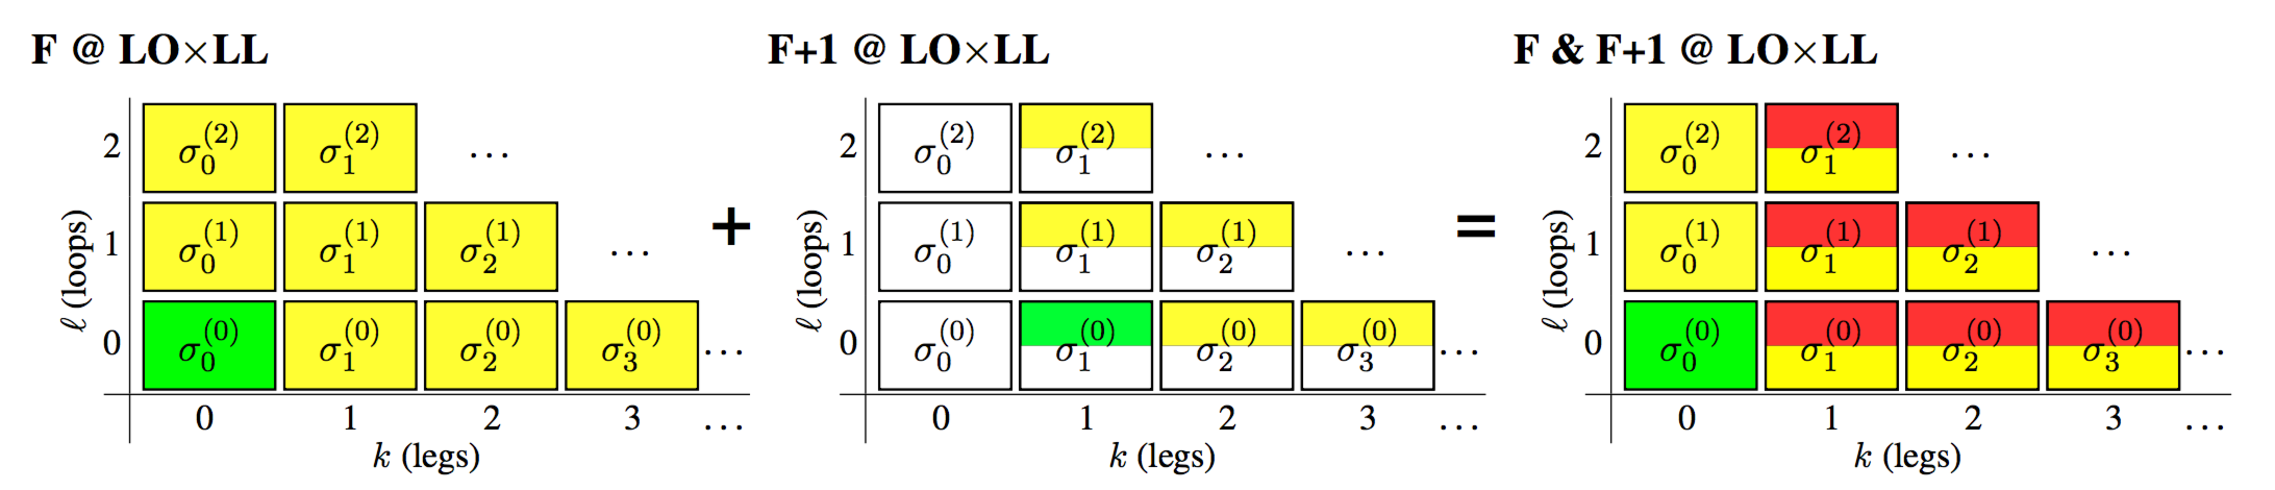
\includegraphics[width=\textwidth]{figures/simul/matching}
\end{center}
\caption{Illustration of the source of possible double-counting originating from adding \glspl{me} with different number of legs. Figure from Ref. \cite{Skands:2011pf}.}
 \label{fig:sim:matching}
\end{figure}

Different methods have been designed to match \glspl{me} to showers such that, for each order in perturbation theory, double-counting is avoided. The three main strategies are \cite{Giele:2011cb}:
\begin{description}
\item[Unitarity] This approach consists in correcting the shower splitting functions by multiplicative factors obtained as the ratio of \gls{me} to \gls{ps} approximation:
$$
\rm{Matched} = \rm{Approximate}\frac{\rm{Exact}}{Approximate} \; .
$$
\noindent When these correction factors are inserted in the shower evolution, they guarantee that the shower evolution of the process F describes correctly also the F+1 \glspl{me}, without actually adding the F+1 sample. This strategy has traditionally been worked out only for one extra parton emission. 

\item[Subtraction] The subtraction approach consists in correcting the \gls{psh} by the difference between \gls{psh} and \glspl{me}:
$$
\rm{Matched} = \rm{Approximate} + (\rm{Exact}- \rm{Approximate}) \; .
$$

\noindent With this strategy, the corrections are not resummed and the events are weighted. This is the strategy used in \mcatnlo \cite{Frixione:2002ik,Frixione:2003ei,Frixione:2008ym}, and the \Powheg method \cite{Frixione:2007vw} is an hybrid between this and the unitarity approach.

\item[Slicing] The slicing approach divides the phase space into two regions: one described mainly by the \glspl{me} (by vetoing shower emissions below a cutoff scale, the matching scale), and one mainly by the \gls{psh}:
\begin{equation*}
\begin{split}
 {\rm{Matched (above \; matching \;  scale)}} &\approx {\rm{Exact}} (1 + {\mathcal{O}} ( \alpha_s)) \; , \\
{\rm{Matched (below \; matching \;  scale)} } &= {\rm{Approximate}} + ({\rm{Exact}}- {\rm{Approximate}})  \\
& \approx {\rm{Approximate}}    \; ,
\end{split}
\end{equation*}


\noindent where the last approximation holds because, below the matching scale, the \glspl{me} and the \gls{psh} give similar results. 
With the slicing strategy, the corrections are not resummed and the events are weighted, but the weights are all positive. This approach can be extended beyond the first extra emission. 
Examples of this approach are the CKKW \cite{Catani:2001cc} and MLM \cite{Mangano:2006rw,Mrenna:2003if} prescriptions. The MLM approach at \gls{nlo} is known as FxFx \cite{Frederix:2012ps}. 

\end{description}


\subsection{Hadronization}

At the end of the shower we have emissions at very low energy and angles, which correspond to high values of the \gls{qcd} coupling constant. 
When the strong coupling becomes of order unit, the interaction is very strong and this is presumably what gives rise to hadronization, the process where colored partons, after parton shower, become a set of colorless hadrons (primary hadrons), 
that can in turn decay into secondary hadrons. This transition is described through phenomenological models since the hadrinization scale, that corresponds also to the \gls{ir} cutoff of the parton shower, is outside the perturbative regime of \gls{qcd}. At the end of the shower, the color, flavour and momentum distribution is already organized, and the hadronization process can only do a local redistribution.
Two main hadronization models are used in \gls{mc} generators:

\begin{description}
\item[String Model] The string model \cite{Artru:1974hr}, whose schematic is depicted in Figure \ref{fig:string_model}, is based on linear confinement: the potential energy between two colored particles increases linearly with their distance, when the distance is greater than about 1 fm (while at shorter distances also a Coulomb term is present). The term "string model" comprises several different models, among which the most used nowadays is the Lund model \cite{Andersson:1983ia,Andersson:1998tv}. 
A color string forms that joins the the final state in a string configuration of field energies, and hadrons originate from the breakups of the string. The proportionality constant of the linear inter-quark potential can be measured from quarkonia spectra or from lattice \gls{qcd}, and results to be $\approx$ 1 GeV/fm.
The main difference between quarks and gluons resides in the fact that, while quarks are connected to one single string, gluons are connected to two and have therefore a rate for hadron production double than that of quarks. 
% chiara: describe the main steps of the string model hadronization
The fragmentation function determines the probability of a given hadron to carry a certain fraction of the available momentum. In the Lund model the form of the fragmentation function is constrained by the left-right symmetry necessary to make the model independent on the sequence of string breakups. The resulting function depends on the mass and \pt of the hadron, leading to heavier hadrons carrying on average an higher fraction of the momentum.

\item[Cluster Model] The cluster model, sketched in Figure \ref{fig:cluster_model}, is based on preconfinement. The clusters of color and anti-color, instead of forming a string, at a sufficient low scale can decay directly into (possibly unstable) hadrons. The mass distribution of the preconfined clusters results to be independent on the scale and nature of the original hard process. This universal distribution of the cluster mass peaks below 1 GeV, with a tail that extends to above 10 GeV; these cluster with very high mass are decayed as a string.  

\end{description}

\begin{figure}[h]
\begin{center}
  \subfigure[]{
    \label{fig:string_model}
    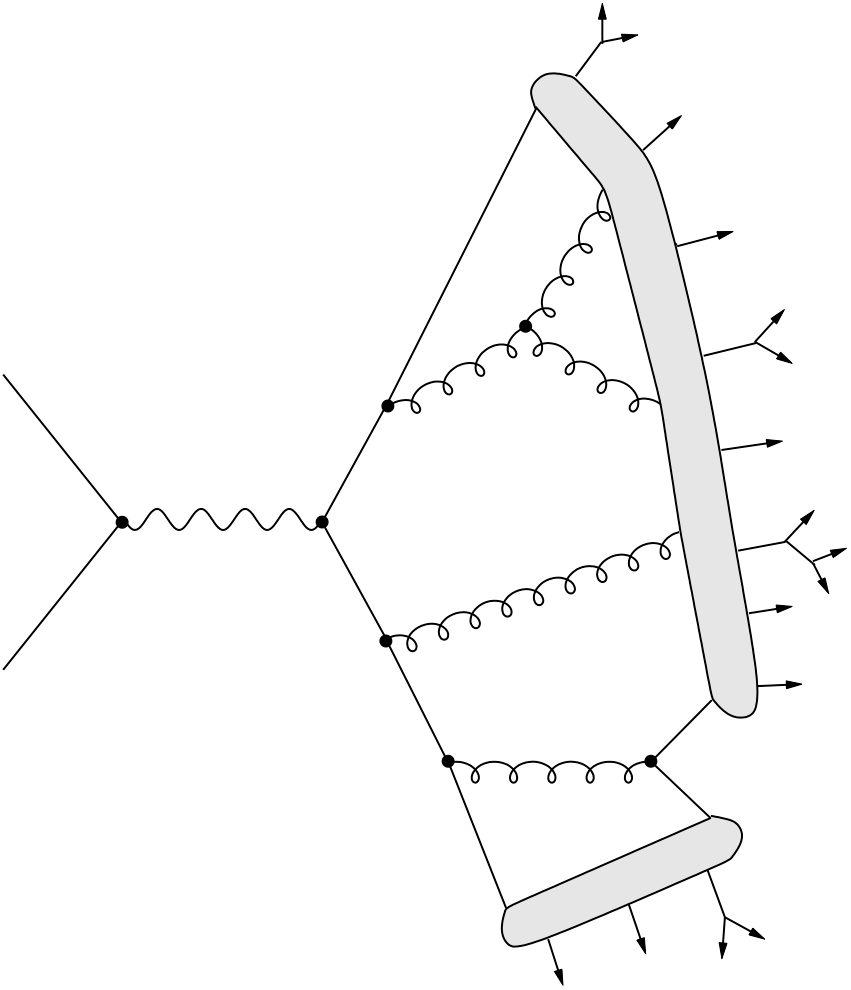
\includegraphics[width=0.35\textwidth]{figures/simul/Figures_MonteCarlo_string_had.pdf}
  }
    \subfigure[]{
    \label{fig:cluster_model}
    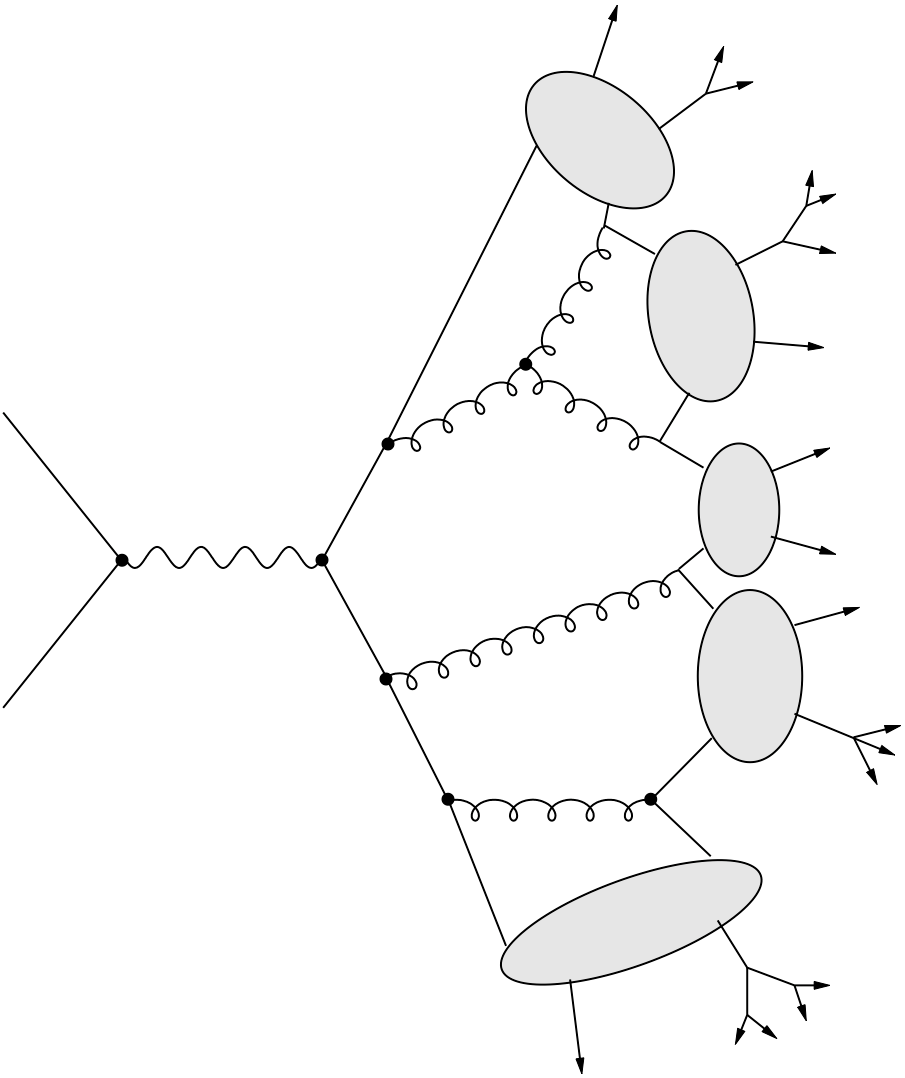
\includegraphics[width=0.35\textwidth]{figures/simul/Figures_MonteCarlo_clustr_had.pdf}
  }
\end{center}
% chiara note: check reference!
 \caption{Schematic view of string hadronization model \subref{fig:string_model} and cluster hadronization model \subref{fig:cluster_model}. Figure from Ref. \cite{Isildak:2013kfa}.}
  \label{fig:had_model}
\end{figure}


These two hadronization models have been developed in the 1980's, and since then there has been no fundamental progress in the theoretical understanding of hadronization. 
When the simulation of the events stops before hadronization, it is referred to as "parton-level".

\subsection{Underlying event}

Protons contain more than one parton; the partons that do not participate to the hard scattering can undergo interactions as well, giving origin to multiple parton interactions in the same collision (underlying event).
These secondary interactions are in general of lower momentum, since the \glspl{me} is larger for low momentum transfer, and will contribute to the activity along the beam direction, less in the transverse plane. 
When the two protons pass through each other the likelihood of having multiple interactions depends on the overlap between the two protons. 
To model the underlying event, the assumption is made that these processes are $2\rightarrow2$ scattering; the \glspl{me} for these diverges at small angle, so the modelling is dependent on the chosen \pt cutoff. 
Because of the low-\pt nature of the underlying event, its description is based on phenomenological models \cite{ATL-PHYS-PUB-2014-021,Skands:2010ak}.
To model the data, color reconnection between the primary interaction and the underlying event is needed. 

\subsection{Pileup}

The term pileup refers to additional \gls{pp} interactions happening in the same bunch crossing (in-time pileup) or in events in different bunch crossings (out-of-time pileup). 
The presence of pileup challenges the reconstruction of the event, as it gives rise to extra activity overlapping with the products of the hard-scattering. The techniques used to model in-time pileup are the same as for the underlying event; 
for out-of-time pileup, similar methods are used but simulating the time response of the detector electronics to collisions from the previous bunch crossing. 

\section{Monte Carlo generators}
\label{sec:mcgen}

The simulations described in the above sections are carried out by event generators, that can be either general purpose, 
if they can reproduce all of the steps of the event generation, or specialized to one functionality. 
In this section the main characteristics of the generators used in the analyses described in this thesis are reviewed.

\subsection{General purpose generators}

Several independent codes allow to study the effects of different modelling of the hadronization and different choices for the parton shower. The three main general-purpose event generators are:

\begin{description}
\item[\PY] \cite{Sjostrand:2006za,Sjostrand:2014zea} \PY is a general purpose generator that uses \gls{lo} \glspl{me} for $2\rightarrow n $ ($n \leq 3$) processes; 
it is capable to simulate both hard and soft interactions, including \gls{isr} and \gls{fsr} and multiple parton interactions.
It uses a \pt-ordered parton shower and the Lund string hadronization model. It is commonly used as a \gls{psh} generator, interfaced with a different generator that computes the \glspl{me}.

\item[\HW] \cite{Corcella:2000bw,Bahr:2008pv,Bellm:2015jjp} It computes $2\rightarrow 2$ \gls{lo} \glspl{me}.
 The partons shower is ordered by the anlge of the emitted parton. Gluon splitting processes ($g \rightarrow q\bar{q}$ and $g \rightarrow gg$) in the collinear approximation are not symmetric in the azimuthal direction due to interference of positive and negative helicity states in the original gluon. 
While \PY uses a method that takes these affects into account only partially \cite{Webber:1987uy}, \HW uses one that fully includes spin correlations \cite{Collins:1987cp}. The hadronization is based on the cluster model.

\item[\Sherpa] \cite{Gleisberg:2008ta} The \Sherpa event generator can provide multi-leg \glspl{me} both at \gls{lo} (up to four extra partons) and at \gls{nlo} (up to two extra partons). 
The matching between \glspl{me} and the dipole-type parton shower \cite{Schumann:2007mg} follows the CKKW prescription.
It uses a cluster hadronization model. 

\end{description}

The recent versions of all three generators are coded in c++, but \HW and \PY were originally developed in Fortran.  

\subsection{Matrix elements generators}

The generators described in this section do not provide a full description of the event, but aim instead at improving the 
computation of the \glspl{me}, and can be afterwards interfaced to a general purpose generator to simulate parton shower, underlying event and pielup. The most common \glspl{me} generators are:

\begin{description}
\item[\PowhegBox] \cite{Alioli:2010xd} In this framework it is possible to implement \gls{nlo} \glspl{me} computations, using the 5 flavour scheme.
It uses the \Powheg method for matching. 

\item[\aNLO] \cite{Alwall:2014hca} This generator can compute \glspl{me} at \gls{lo} for any user-specified lagrangian, and at \gls{nlo} accuracy for selected processes. It includes up to two additional partons and is then interfaced to a parton shower using the CKKW-L method. 

\end{description}

\subsection{Specialized generators}

The specialized generators provide a better description of one specific aspect of the \gls{mc} simulation. Some of them are:

\begin{description}
\item[\evtgen] \cite{Lange:2001uf} This package simulates the decay of heavy flavour particles, in particular B and D hadrons. 
In the simulation of the decay it uses decay amplitudes instead of probabilities and it includes spin correlations. 
When interfaced with other event generators, it can be used to re-decay the heavy flavour particles, substituting the more sophisticated decay chains simulated by \evtgen to the original ones.

\item[\tauola] \cite{Jadach:1990mz} General purpose event generators treat tau leptons as stable particles. 
The tau decays are then handled by separated packages like \tauola, which includes leptonic and semileptonic decays, paying attention to the tau polarization. Since the format of the tau-related information is generator-dependent and the results of the original generator need to be replaces, also the input and output formats of \tauola depend on the generator it is interfaced with.

\item[\photos] \cite{Barberio:1990ms} This generator handles electromagnetic radiation, estimating the size of the \gls{qed} bremsstrahlung in the collinear approximation, and is used by \tauola. 


\end{description}


\section{Detector simulation}
\label{sec:detsim}

The outcome of the event simulation are the four-vectors of all the stable particles produced in the final state of the event, stored in the standard HepMC format \cite{Dobbs:2001ck}.
When this information is used directly, the analysis is referred to as "particle level" analysis; furthermore, if we want to filter the simulated events based on the final state, this can be done at this stage. 
While the event generation can already provide information on the kinematic of the event, it is not enough to compare the \gls{mc} simulations with the 
data collected by the \gls{atlas} detector. 
After the event simulation, the \gls{atlas} simulation chain \cite{Aad:2010ah} (described in Figure \ref{fig:sim:chain}) proceeds with the emulation of the
interaction of the particles with the detector and the signal generated in each of the detector's subsystems, 
which is done with the \geant package \cite{Agostinelli:2002hh}. The configuration of the detector, including any misalignment, can be set at run time, and the energy depositions are recorded as hits. The digitalization step takes the input hits from the hard scattering, underlying event and pileup and transforms them into detector signals, adding also detector noise. Also the response of the \gls{lone} trigger (described in Section \ref{sec:cern:trigger}) is simulated at this stage. The final output of the digitalization is the \gls{rdo} file, to which the output of the \gls{atlas} detector itself, which is in "bytestream" format, can be converted as well. The \gls{hlt} decision and the event reconstruction run on the \gls{rdo} data format. After the detector simulation, the \gls{mc} simulated events are treated in the same manner as data, going through the object reconstruction procedures
describes in Chapter \ref{sec:event:reco}.

\begin{figure}[h]
\begin{center}
    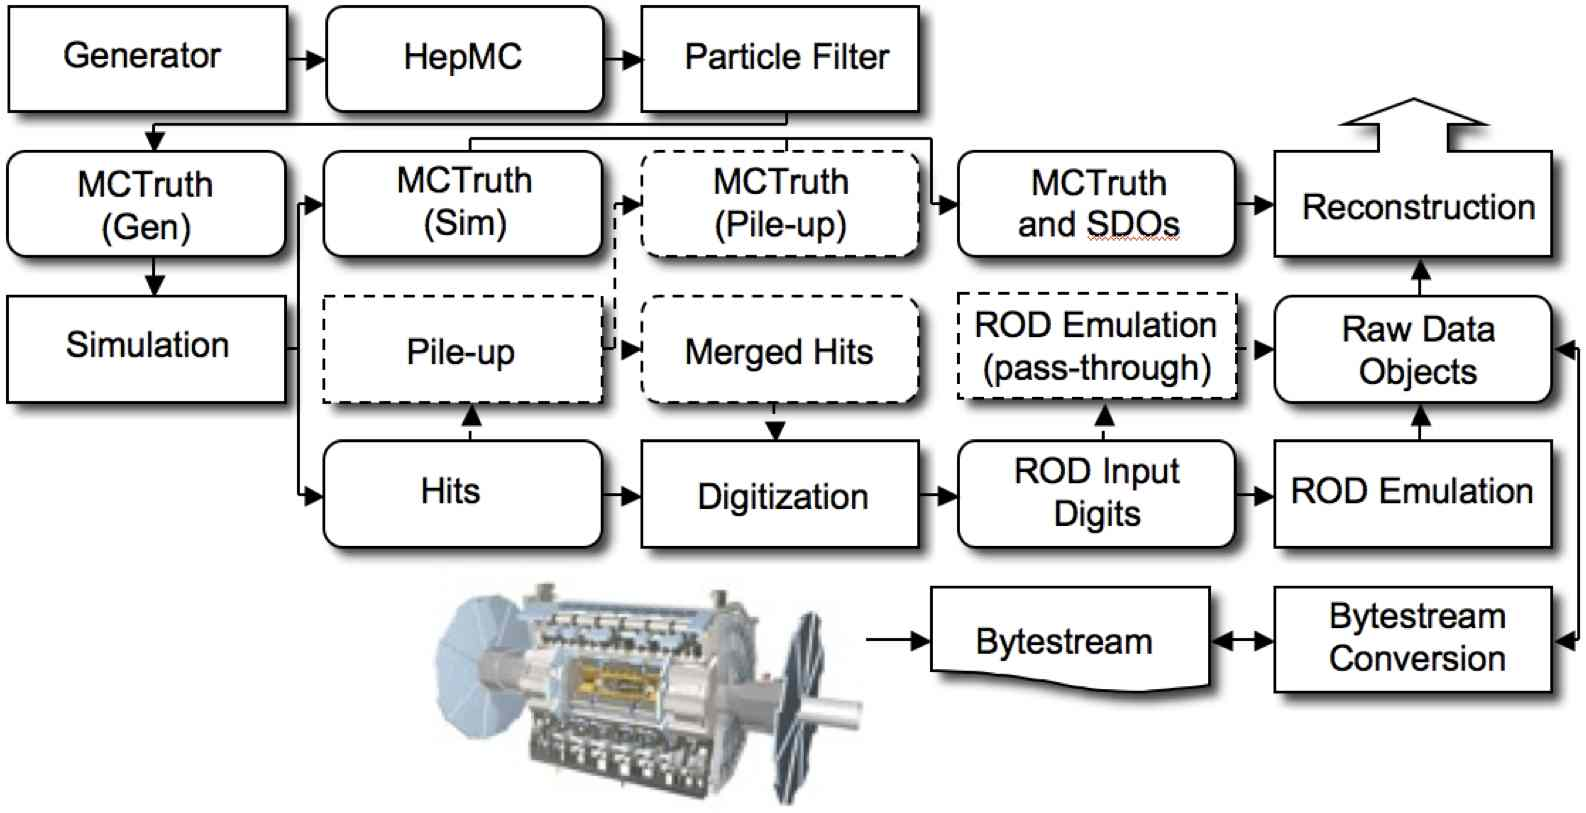
\includegraphics[width=0.8\textwidth]{figures/simul/outline_v2}
\end{center}
\caption{The \gls{atlas} simulation software, compared with the processing of the recorded data; square-cornered boxes represent algorithms, while data objects are represented as rounded boxes. Figure from Ref. \cite{Aad:2010ah}.}
 \label{fig:sim:chain}
\end{figure}

The full simulation of the interaction of particles with the \gls{atlas} detector is a CPU-intensive task. 
ATLFAST-II \cite{Aad:2010ah} is a fast simulation method aiming at simulating the large amount of \gls{mc} events required by \gls{atlas} analyses by making use of a simplified detector description. 
ATLFAST-II has two components: the Fast ATLAS Tracking Simulation (Fatras) \cite{Edmonds:2008zz}, to emulate the response of the \gls{id} and of the muon system, 
and the Fast calorimeter Simulation (FastCaloSim) \cite{ATLAS:1300517}, that takes care of the simulation of the calorimeters. The default ATLFAST-II simulation uses the full \geant simulation for the \gls{id} and the muon spectrometer, 
while it uses FastCaloSim to emulate the energy deposited in the calorimeters using a parametrization of the longitudinal and lateral energy profile. 
ATLFAST-IIF uses both FastCaloSim for the calorimeters and Fatras for the tracking systems. 
The output of ATLFAST-II includes all the properties necessary to run the same event reconstruction as with \geant or the real data.



\section{Data-driven corrections}
\label{sec:datacorr}

After begin simulated, the \gls{mc} events are normalized to the highest-available-order cross-section, and are reweighted so that the simulated pileup distribution matches the one observed in the data that will be compared with the simulation.
Despite the accurate simulation, residual differences can be present in the reconstruction and selection efficiency in data and \gls{mc} simulation. 
These differences are corrected for by multiplying the \gls{mc} simulation by \glspl{sf}, defined as the ratio of the efficiency (of a reconstruction or a selection) in data and \gls{mc}:
\begin{equation}
{\rm SF} = \frac{\epsilon_{\rm data}}{\epsilon_{\rm MC}} \; .
\end{equation}
\noindent These \glspl{sf} can be function of the kinematic of the objects in the event (often \pt and $\eta$). 
Some examples of \glspl{sf} for the objects relevant for the analyses described in this thesis are given in Chapter \ref{sec:event:reco}.




